\documentclass{article}

\usepackage{booktabs}
\usepackage{multirow}
\usepackage{amsmath}
\usepackage{hyperref}
\usepackage{overpic}
\usepackage{amssymb}
\usepackage{lipsum}

\usepackage[accepted]{dlai2021}

%%% STUDENTS: FILL IN WITH YOUR OWN INFORMATION
\dlaititlerunning{Ornithology expert system}

\begin{document}

\twocolumn[
%%% STUDENTS: FILL IN WITH YOUR OWN INFORMATION
\dlaititle{BirdCLEF2021: An ornithology expert system}

\begin{center}\today\end{center}

\begin{dlaiauthorlist}
%%% STUDENTS: FILL IN WITH YOUR OWN INFORMATION
\dlaiauthor{Edoardo De Matteis}{}
\end{dlaiauthorlist}

%%% STUDENTS: FILL IN WITH YOUR OWN INFORMATION
\dlaicorrespondingauthor{Edoardo De Matteis}{dematteis.1746561@studenti.uniroma1.it}

\vskip 0.3in
]

\printAffiliationsAndNotice{}

\begin{abstract}
We approach the BirdCLEF2021 bird classification task and see how we can train a good ornithology expert system with only soundscape recordings, thus making no use of most of the dataset.
The code is available on GitHub at \href{https://github.com/edodema/Birdcalls}{https://github.com/edodema/Birdcalls}
\end{abstract}

\section{Introduction}
Birds are high up in the food chain, this means that are sensitive to changes in the ecosystem and monitoring them can give us informations about pollution and the environment as a whole ~\cite{becker2003biomonitoring}.
Small birds are often difficult to sight and easy to hear, their calls are generally characteristic of each species so can be used for identification.
Our goal is to listen to ambient recordings and guess birds' species through their calls, the task is set up as an image classification among $n+1$ classes i.e. $n$ species plus no bird being detected. 

\paragraph*{Dataset.}
The BirdCLEF2021 dataset contains both recordings of birds in a controlled environment and noisy soundscapes tracks, we will use only the latter.
Tracks are split by 5 seconds  windows and labeled with primary and secondary gold truths - among other privileged data - but for our purposes we will consider primary ones only; we are being conservative so that should not be a problem.

\section{Related work}
Many previous works exploit spectrograms to reduce audio tasks to image ones ~\cite{hamdyaudio} ~\cite{michelashvili2020denoising} ~\cite{xie2021audio}, among them ~\cite{xie2021audio} uses recurrent layers to deal with sequential knowledge.
With the same intent we employ attention layers in one of the basic blocks that will form our model - inspired by ~\cite{zhang2020resnest}.
Some tweaks to stabilize image feature extraction have been taken by \textit{ResNet} ~\cite{he2016deep}.

\section{Method} \label{sec:method}
What happens when ornithologists recognize a birdcall, do they first detect a sound to then focus on classifying it or does their brain automatically do that subconsiously?
It makes sense to believe it is possible to be so proficient to unconsciously recognize birds, as already happens with familiar sounds ~\cite{kirmse2009familiarity}. 
I tried both the approaches but only the "subconscious" one is covered here due to computational issues with the other.

\paragraph*{Preprocessing.}
The dataset is highly unbalanced (figure \ref{fig:soundscapes_classification_freq}) 
so it was augmented by random oversampling and each 5 seconds frame is encoded as a spectrogram in mel scale.
In audio samples there can be both plain ambient noise and birds chirping, thus transforming spectrograms (e.g. by random crops) can lead to wrong labeling, besides that, I also wanted to avoid data losses due to this type of knowledge being sequential.

\begin{figure}
    \centering
    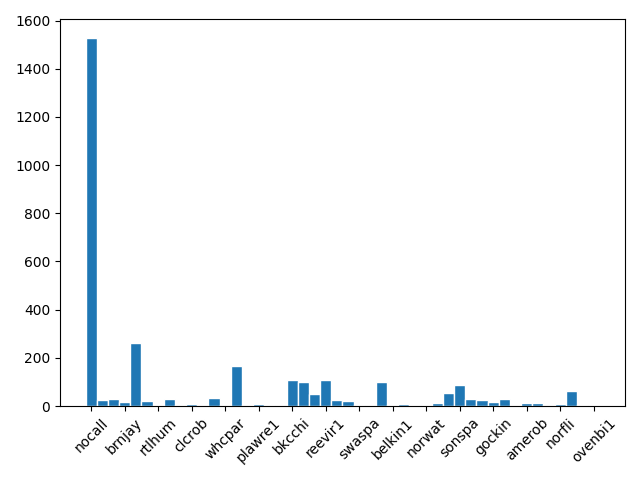
\includegraphics[scale=.35]{images/soundscapes_distribution_birds.png}
    \caption{Primary label distribution in soundscape recordings.}
    \label{fig:soundscapes_classification_freq}
\end{figure}

\paragraph*{CNNAtt.}
This seq2seq layer expolits attention to grasp that sequential knowledge: the spectrogram passes through three different convolution pipelines with each one being the query, key and value for the attention, it takes inspiration by a \textit{ResNeSt} block ~\cite{zhang2020resnest} with 3 fixed cardinals. 
Self-attention layers  work on tensor rows independently, looking at frequencies with no connection between them, thus a second attention layer works on spectrograms feature images' transpose; the two representations are then concatenated to a 2 channel image.
When we refer to a CNNAtt$k$ convolutions have all the same kernel size $k$.

\begin{figure}
    \centering
    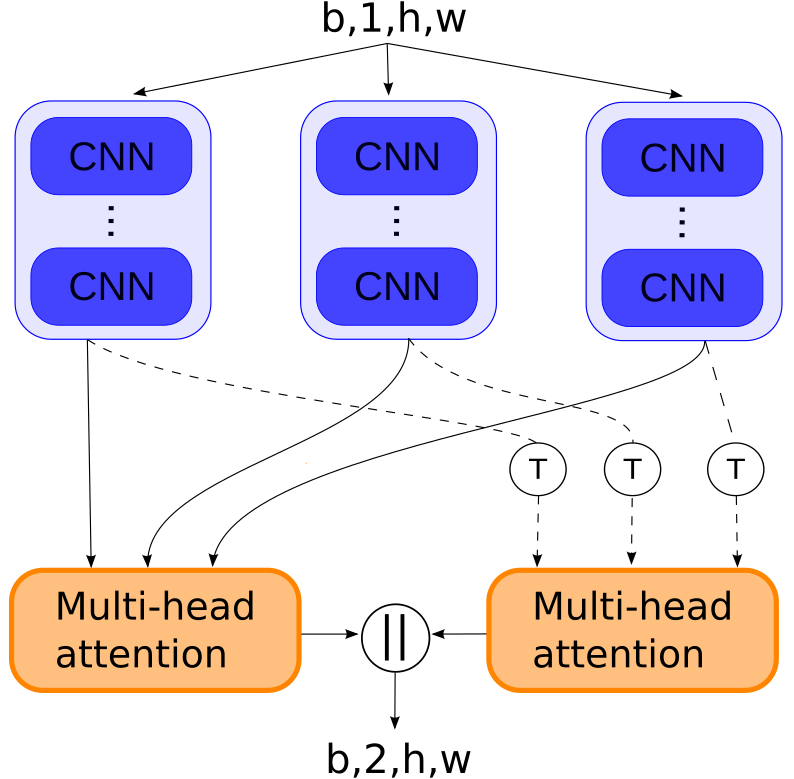
\includegraphics[scale=.3]{images/cnn_att.png}
    \caption{A CNNAtt block.}
    \label{fig:cnnatt}
\end{figure}

\paragraph*{CNNRes.}
Residual networks help reducing errors in deep networks, this architecture employs six convolutions of the same kernel size with three skip connections between them (figure \ref{fig:cnnres}), $n$ layers can be stacked one on top of the other and we call it CNNRes$n$.
As a rule the number of kernels stays the same when the input image and the feature map have the same size, it is doubled when the latter is half the first to preserve complexity ~\cite{he2016deep}.
Between two different CNNRes block there are no connections thus no dealing with different dimensionalities. 

\begin{figure}
    \centering
    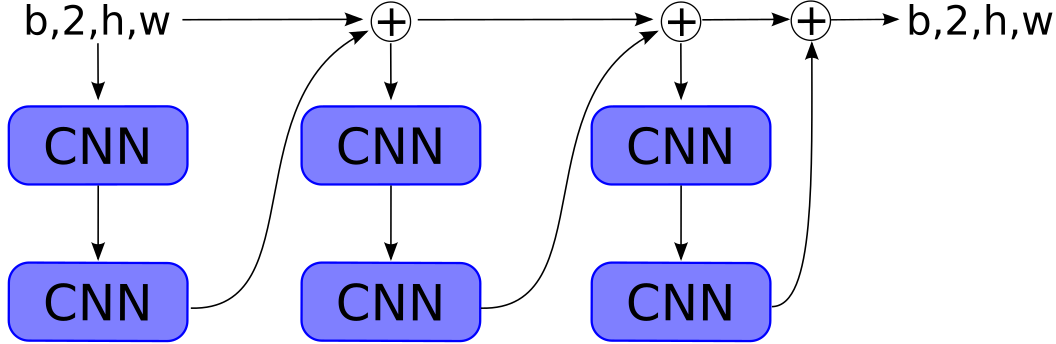
\includegraphics[scale=.25]{images/cnn_res.png}
    \caption{A CNNRes block.}
    \label{fig:cnnres}
\end{figure}

The aforementioned layers build up the feature extraction backbone, a convolution between CNNAtt and CNNRes are needed to deal with the number of filters.
After that we have $m$ bilinear GRU layers to extract causal knowledge, and last a linear layer to output logits.
When defining models for out experiments we can ignore these last two heads due to them being common to all of them.

\section{Results and conclusions}
In our experiments we will use CNNRes2 (with kernel sizes $3$ and $5$) and CNNAtt5CNNRes2 models, according to the previously defined rules, we also fine-tune pretrained models \textit{ResNet18} and \textit{ResNet50}, in which we add a convolution and a linear layer to match \textit{ResNet}s input and output.
Optimization is done by \textit{Adam} algorithm on a cross entropy loss with small batches, both to gain a regularizing effect and because of memory limitations.
Results are reported in table \ref{tab:joint-results}, a small learning rate is needed to stabilize descent due to the high variance of 8-sampled batches.
Since datasets have been balanced and all classes are equally important it makes sense to use accuracy.

From the results we can confirm that convolutional neural networks do wonders when priors apply, while training attention is not worth the hassle. 
Occam's razor holds and simpler residual networks seem to be better than fine-tuned models, yet we are transferring knowledge so we cannot say that with certainty. 

\begin{table}
    \caption{Performances for the validation set on 20 epochs with fixed seed, the test accuracy is reported for CNNRes2 only.}
    \label{tab:joint-results}
    \begin{center}
        \begin{small}
            \begin{tabular}{p{0.35\linewidth} | ccc}
                \toprule
                & \multirow{2}{0.13\linewidth}{LR} 
                & \multirow{2}{0.13\linewidth}{Loss $\downarrow$} 
                & \multirow{2}{0.13\linewidth}{Acc. $\uparrow$} \\
                Model \\
                \midrule
                ResNet50 & 1e-4 & .52 & 82.3\% \\
                ResNet18 & 1e-4 & .21 & 92.2\% \\
                ResNet18 (frozen) & 1e-4 & 1.03 & 71.6\% \\
                CNNRes2 & 1e-4 & \textbf{.02} & \textbf{99.1\%} \\
                CNNAtt5 + CNNRes2 & 1e-4 & .04 & 98.7\% \\
                \midrule
                \midrule
                Test & - & - & 99.4\% \\
                \bottomrule
            \end{tabular}
        \end{small}
    \end{center}
    \vspace{-0.5cm}
\end{table}

\begin{figure}
    \centering
    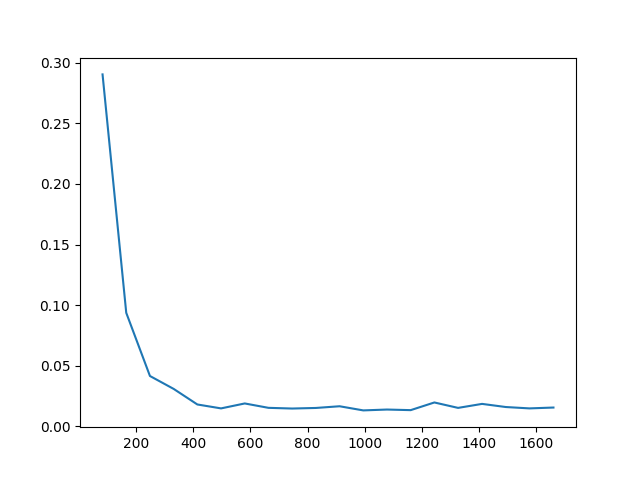
\includegraphics[scale=.5]{images/val_loss.png}
    \caption{Validation loss for CNNRes2GRU1FC1.}
    \label{fig:val-loss}
\end{figure}

\paragraph*{Future works.}
Adding a threshold to consider secondary labels too, train on the whole dataset to see if it yields some improvement and train the "conscious" model (section \ref{sec:method}) to compare results.

\bibliography{references.bib}
\bibliographystyle{dlai2021}

\end{document}